% ComptonScatteringSpectra
\documentclass[draftcls,onecolumn]{IEEEtran}

%% INCLUDING THE PREAMBLE
%%%%%%%%%%%%%%%%%%%%%%%%%%%%%%%%%%%%%%%%%%%%%%%%%%%%%%%%%%%%%%%%%%%%%%%%%%%
%                                                                         %
%                                 PREAMBLE                                %
%                                                                         %
%%%%%%%%%%%%%%%%%%%%%%%%%%%%%%%%%%%%%%%%%%%%%%%%%%%%%%%%%%%%%%%%%%%%%%%%%%%

%% PACKAGES
\usepackage[]{lineno}
%\linenumbers
\usepackage[usenames,dvipsnames]{xcolor}
\usepackage{microtype}
\usepackage[obeyDraft]{todonotes}
\usepackage{fancyvrb}
\VerbatimFootnotes
\usepackage{algorithmic}

%% GRAPHICS RELATED
\usepackage{graphicx}
\usepackage[outdir=./tmp/]{epstopdf}
\graphicspath{{../images/}{./}{./tmp/}}
\DeclareGraphicsExtensions{.eps, .pdf, .jpeg, .png,}

%% CPATION SETUP
\usepackage{float}
\usepackage{caption}
\usepackage{subcaption}
\captionsetup{belowskip=12pt,aboveskip=4pt}


%% BIBLIOGRAPHY
\bibliographystyle{ieeetr}

%% UNITS
\usepackage{siunitx}

%% EQUATIONS
\usepackage{amsmath}
%\numberwithin{equation}{section}

%% HYPERLINKS
\usepackage[debug]{hyperref}

%%%%%%%%%%%%%%%%%%%%%%%%%%%%%%%%%%%%%%%%%%%%%%%%%%%%%%%%%%%%%%%%%%%%%%%%%%%
%                                                                         %
%                             Listing Setup                               %
%                                                                         %
%%%%%%%%%%%%%%%%%%%%%%%%%%%%%%%%%%%%%%%%%%%%%%%%%%%%%%%%%%%%%%%%%%%%%%%%%%%
\usepackage{listings}
\lstset{ %
    language=C++,
    basicstyle=\footnotesize\ttfamily,
    numbers=left,
    numberstyle=\tiny\color{gray},
    stepnumber=2,
    numbersep=5pt,
    backgroundcolor=\color{white},
    showspaces=false,
    showstringspaces=false,
    showtabs=false,
    frame=single,
    rulecolor=\color{black},
    tabsize=2,
    breaklines=true,
    breakatwhitespace=false,
    title=\lstname,
    keywordstyle=\color{blue},
    commentstyle=\color{OliveGreen},
    stringstyle=\color{orange}
}
\DeclareCaptionFont{white}{\color{white}}
\DeclareCaptionFormat{listing}{\colorbox[cmyk]{0.43, 0.35, 0.35, 0.01}{\parbox{\dimexpr\textwidth-2\fboxsep\relax}{#1#2#3}}}
\captionsetup[lstlisting]{format=listing,labelfont=white,textfont=white,singlelinecheck=false,margin=0pt,font={bf,footnotesize}}
%\lstnewenvironment{code}[1][]%
%{ \noindent\minipage{\linewidth}
%	\lstset{#1}
%}
%{\endminipage}
%% USER COMMANDS
\usepackage{isotope}
\newcommand{\iso}{\isotope}
\newcommand{\figurewidth}{\textwidth}
\newcommand{\micron}{$\mu$m}



%% Start of the document
\begin{document}
\title{GEANT4 Simulate Ranges}
\author{Matthew J. Urffer}
\date{\today}
\maketitle

% Nomenclature
\printnomenclature

% Tables of Contents, Figures, Tables
\listoftodos
\tableofcontents
\listoffigures
\listoftables
\lstlistoflistings

\section{Introduction}
Accurate knowledge of the range of a particle in a material is essentail for for the optimal design of a detector.
Knowing the range allows for the selective optimization of the energy deposition by making the detector material thick enough such that all of the particle will be stopped in the material, thus depositing all of it's energy.
Tabulated ranges exists for common materials, and codes such at TRIM and GEANT4 can be used for the calcuation of the range in differnet materials\cite{berger_estar_2005}.

\section{Methods}
The GEANT4 toolkit contains detailed electromagnetic models that can be adapted to calculate the ranges of primary particles.
An example provided with the toolkit, \verb+TestEm1+, provides the basis for calculating the ranges of electrons in aluminum. 
This work adapted that example for calculation of the ranges of in materials that are intresting for polymeric neutron detectors; namely \iso[6]{LiF} loaded polystyrene (PS), \iso[6]{LiF} loaded polyethylnapthalate (PEN), \iso[10]{B} loaded methylstyrene (MS), and \iso[6]{LiF} loaded zinc sulfide (EJ-426HD2).


\subsection{Validation Results}
\label{sec:ValResults}
\autoref{fig:AlphaRangeVal} and \autoref{fig:ElectronRangeVal}

The data was compared to the TRIM calculations preformed by Andrew Mabe.
\subsection{Range of Selected Particles and Ions}
\label{sec:RangeResults}


\end{document}
\begin{figure}
	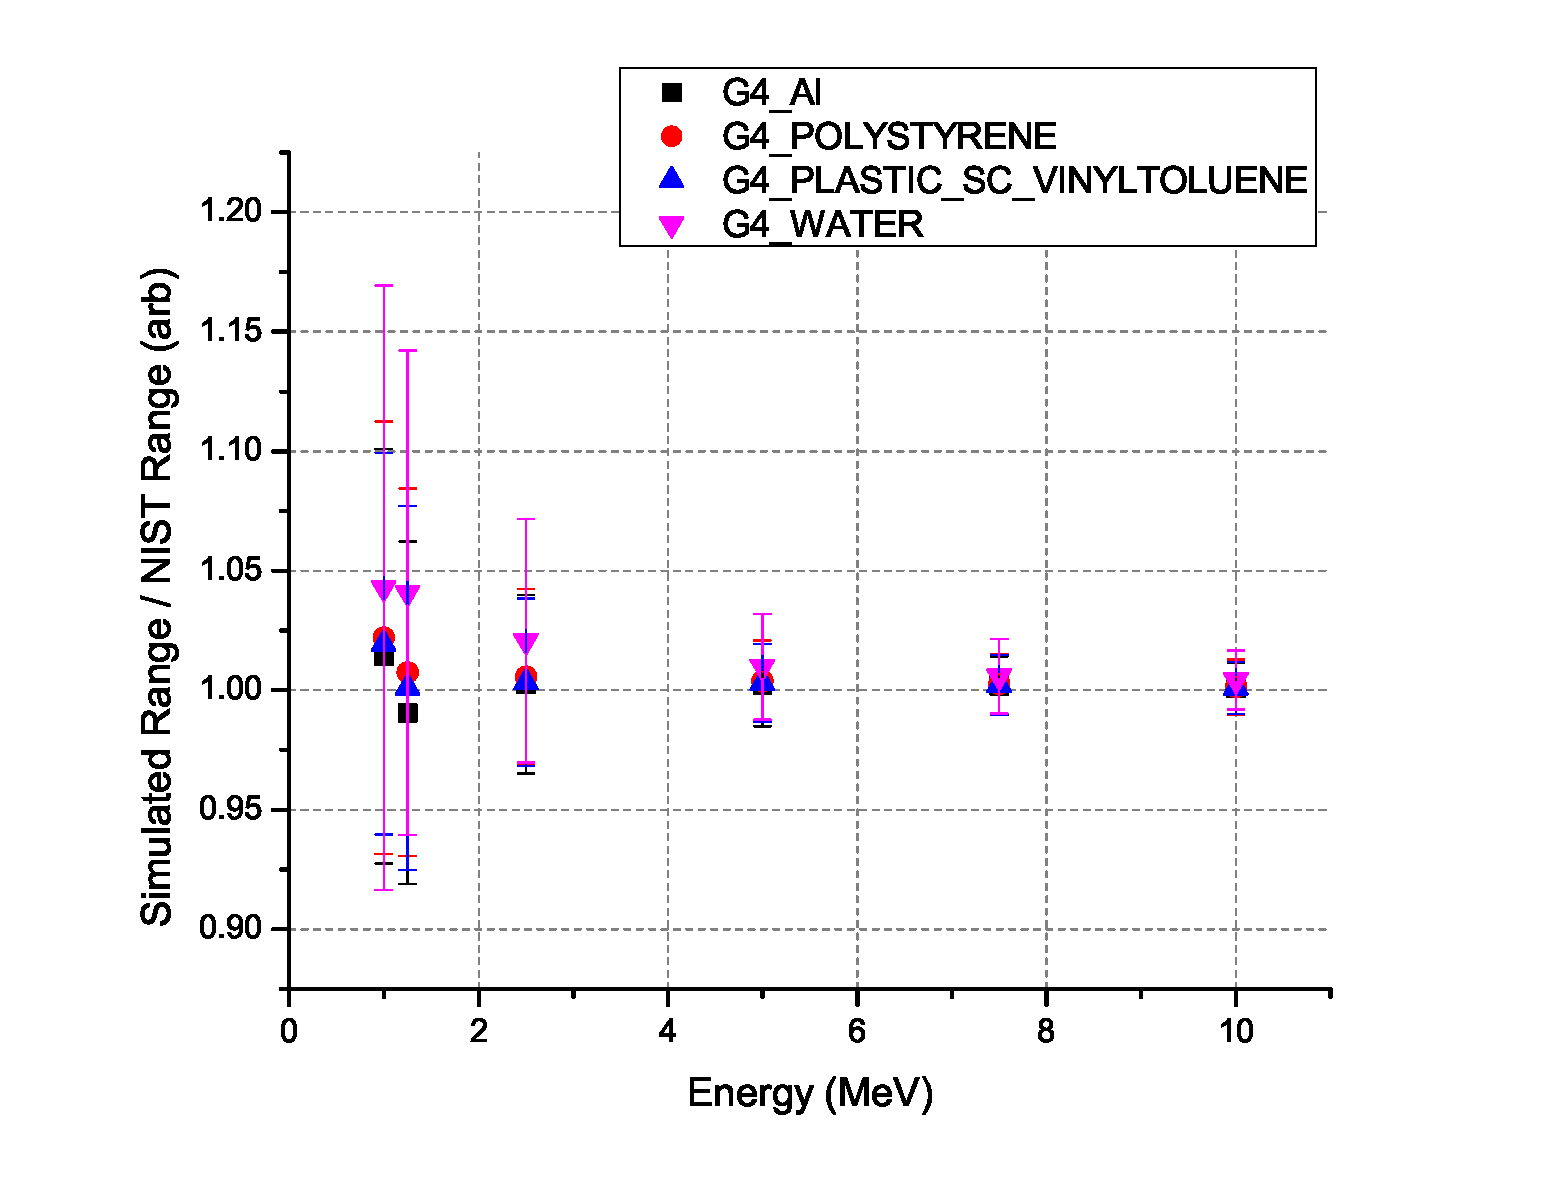
\includegraphics[width=\textwidth]{RangeSim_AlphaVal}
  \caption[Alpha Range Verication]{Comparison of the GEANT4 simulated alpha range to the NIST CSDA range for selected materials.}
  \label{fig:AlphaRangeVal}
\end{figure}
\begin{figure}
  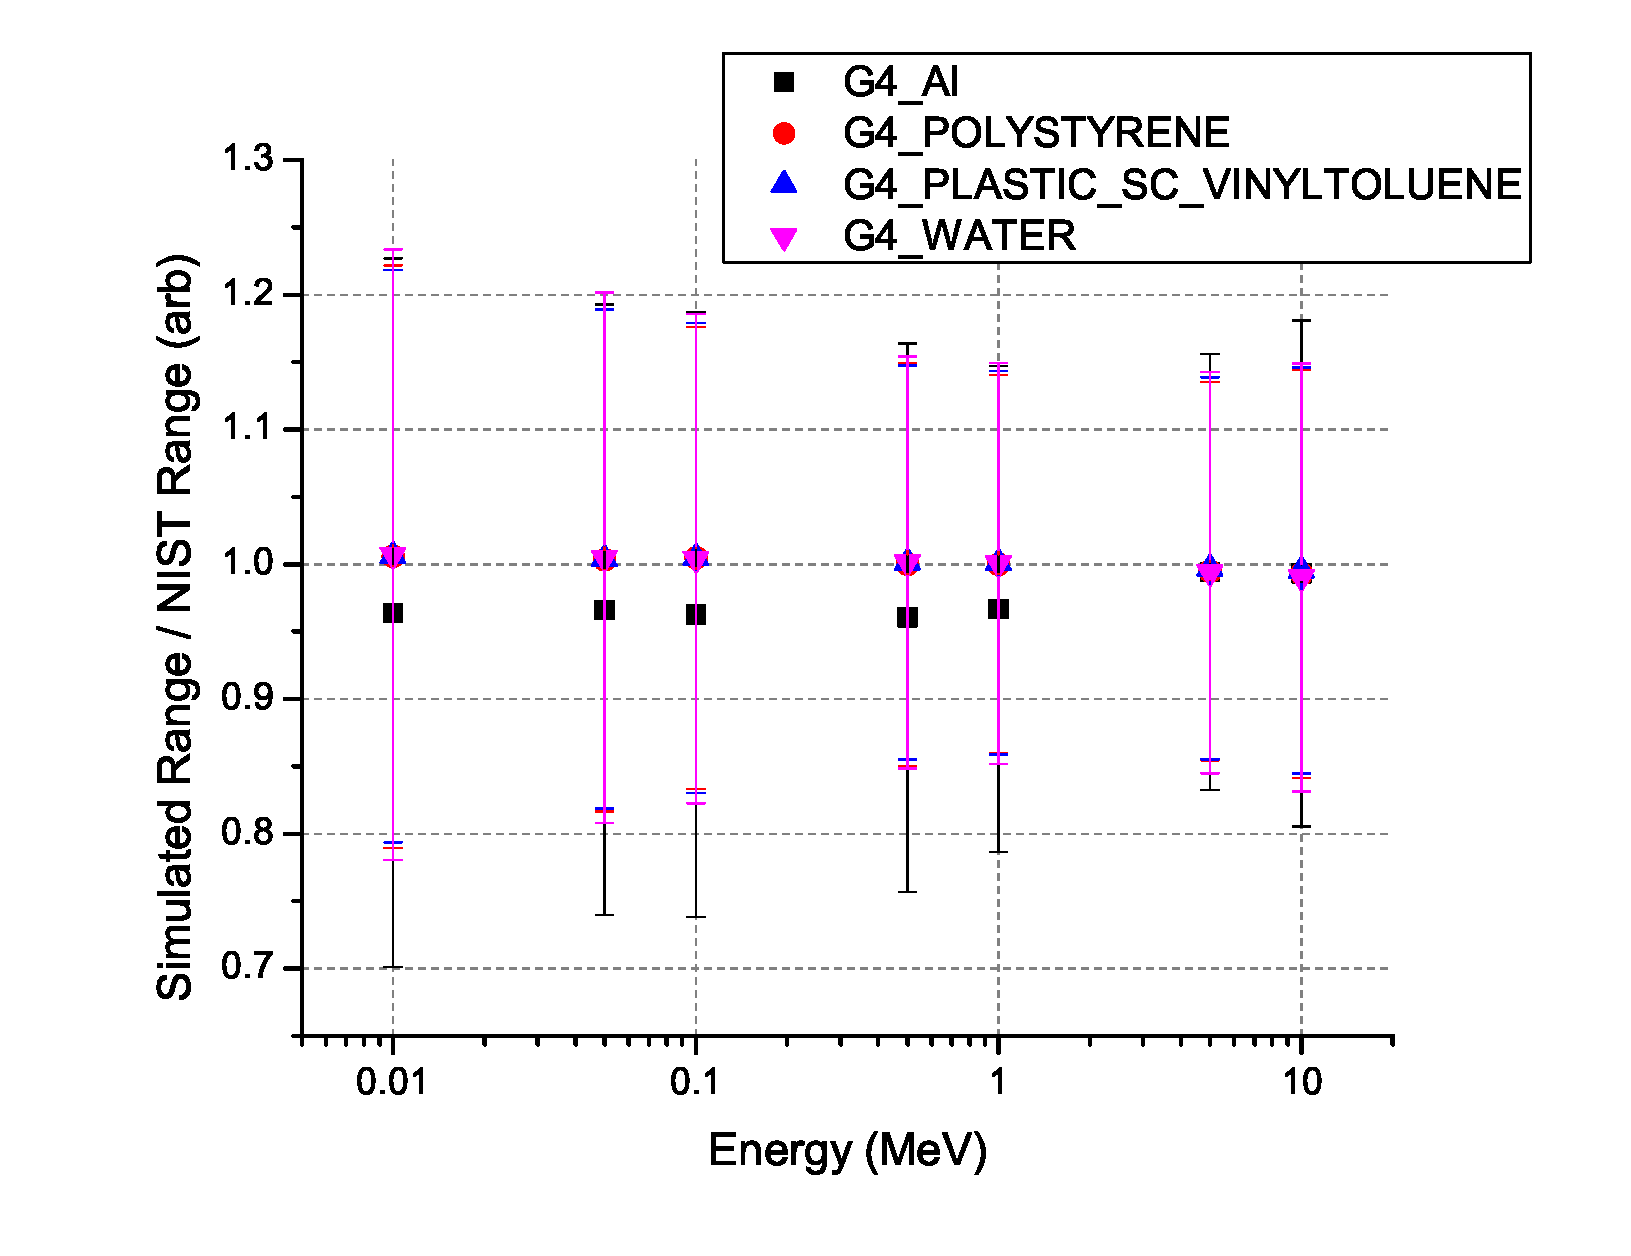
\includegraphics[width=\textwidth]{RangeSim_ElectronVal}
  \caption[Electron Range Verification]{Comparison of the GEANT4 simulated electron range to the NIST CSDA range for selected materials.}
  \label{fig:ElectronRangeVal}
\end{figure}
\begin{figure}
  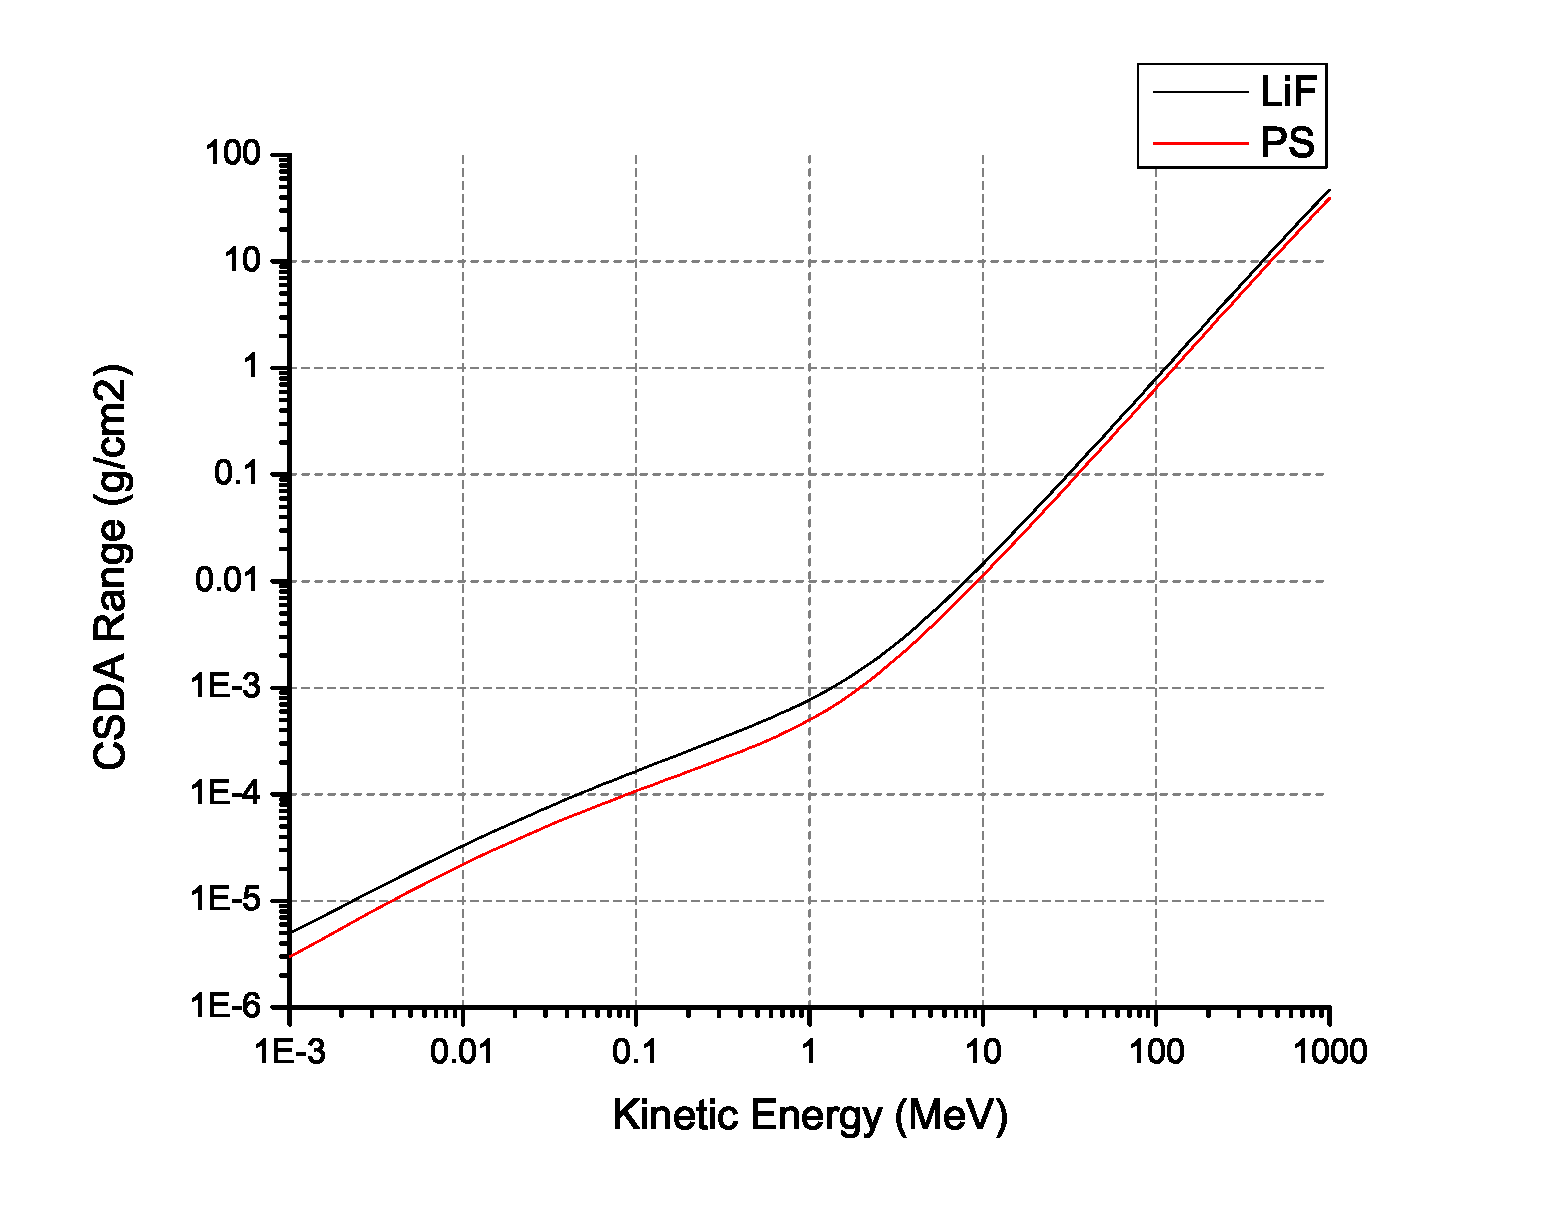
\includegraphics[width=\textwidth]{RangeSim_CSDA-NIST_PS_LiF}
  \caption[Comparison of alpha ranges in LiF and PS]{Comparison of alpha CSDA ranges in PS and LiF. LiF generally has a higher range than PS. Data from NIST ASTAR\cite{berger_estar_2005}.} 
  \label{fig:NISTPSLiF}
\end{figure}
\begin{figure}
  \includegraphics[width=\textwidth]{
  \caption
  \label
\end{figure}
\begin{figure}
  \includegraphics[width=\textwidth]{
  \caption
  \label
\end{figure}
\begin{figure}
  \includegraphics[width=\textwidth]{
  \caption
  \label
\end{figure}
RangeSim_MassFraction_Alpha.eps
RangeSim_MassFraction_Triton.eps
RangeSim_Proj-NIST_Z.eps
